\newcounter{row}
\newcounter{col}
\newcommand\setrow[3]{
  \setcounter{col}{1}
  \foreach \n in {#1, #2, #3} {
    \edef\x{\value{col} - 0.5}
    \edef\y{3.5 - \value{row}}
    \node[anchor=center] at (\x, \y) {\n};
    \stepcounter{col}
  }
  \stepcounter{row}
}

%  
\tikzstyle{module}=[draw, draw=blue!80, text width=10em, 
    text centered, minimum height=5em, minimum width = 15em, drop shadow, rounded corners,
    fill=blue!30]
    
\tikzstyle{block} = [rectangle, draw, fill=blue!30, 
     text width=5em,text centered, rounded corners, minimum height=4em, minimum width = 5em]
\tikzstyle{block1} = [rectangle, draw, fill=white!20, 
     text width=5em,text centered, rounded corners, minimum height=4em, minimum width = 5em]

\tikzstyle{line} = [draw, -latex']

% Define distances for bordering
\def\blockdist{1}
\def\edgedist{1.5}
  
\begin{figure}			
\begin{center}
\subfloat[]{
\scalefont{0.7}
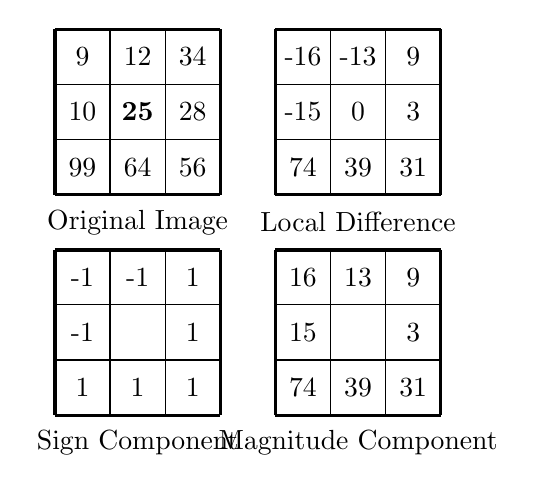
\begin{tikzpicture}[scale=.7]

  \begin{scope}
    \draw (0, 0) grid (3, 3);
    \draw[very thick, scale=3] (0, 0) grid (1, 1);

    \setcounter{row}{1}
    \setrow {9}{12}{34} 
    \setrow {10}{\textbf{25}}{28}  
    \setrow {99}{64}{56}  
    \node[anchor=center] at (1.5, -0.5) {Original Image};
  \end{scope}

  \begin{scope}[xshift=4cm]
    \draw (0, 0) grid (3,3);
    \draw[very thick, scale=3] (0, 0) grid (1,1);

    \setcounter{row}{1}
    \setrow {-16}{-13}{9}  
    \setrow {-15}{0}{3}  
    \setrow {74}{39}{31} 
    \node[anchor=center] at (1.5, -0.5) {Local Difference};
  \end{scope}

  \begin{scope}[yshift=-4cm]
    \draw (0, 0) grid (3,3);
    \draw[very thick, scale=3] (0, 0) grid (1,1);

    \setcounter{row}{1}
    \setrow {-1}{-1}{1}  
    \setrow {-1}{}{1}  
    \setrow {1}{1}{1} 
    \node[anchor=center] at (1.5, -0.5) {Sign Component};
  \end{scope}
  
    \begin{scope}[yshift=-4cm,xshift =4cm]
    \draw (0, 0) grid (3,3);
    \draw[very thick, scale=3] (0, 0) grid (1,1);

    \setcounter{row}{1}
    \setrow {16}{13}{9}  
    \setrow {15}{}{3}  
    \setrow {74}{39}{31} 
    \node[anchor=center] at (1.5, -0.5) {Magnitude Component};
  \end{scope}
\end{tikzpicture}
}\\
\subfloat[]{
\begin{tikzpicture}[node distance = 10cm,scale=0.7, every node/.style={scale=0.7}] % 
    % Place nodes   
\begin{scope}[node distance=10cm]
	\node[block] (CLBPs){ $CLBP_{s}$};
\end{scope}
\node[block,below of=CLBPs , node distance = 3cm] (CLBPm) { $CLBP_{m}$};
\node[block,below of=CLBPm, node distance =3cm] (CLBPc) { $CLBP_{c}$};
\node [block, left of=CLBPc, node distance =4cm] (GL) {Grey level of center};
\node [block, above of=GL, node distance =4cm] (LC) {Local Differences}; 
    
    \begin{pgfonlayer}{background}
	\path (LC.west |- LC.north)+(-0.3,-0.8+\blockdist) node (a) {};
    \path (GL.east |- GL.south)+(+0.3,-0.3) node (b) {};          
    \path[fill=blue!10,rounded corners, draw=blue!20, dashed] (a) rectangle (b);
	\end{pgfonlayer}
	
	\begin{pgfonlayer}{background}
	\path (CLBPs.west |- CLBPs.north)+(-0.3,-0.3+\blockdist) node (c) {};
    \path (CLBPc.east |- CLBPc.south)+(+0.3,-0.3) node (d) {};          
    \path[fill=blue!10,rounded corners, draw=blue!20, dashed] (c) rectangle (d);
	\end{pgfonlayer}
	\path (CLBPs.west |- CLBPs.north) +(+1.05,-0.7+\blockdist) node (bgfea) { Binary Patterns};
	
	\path (CLBPs.east |- CLBPs.north)+(0.2,-0.4+\blockdist) node (i) {};
	\path (CLBPc.east |- CLBPc.south)+(0.2,-0.4) node (j) {};

	\draw[decorate,decoration={brace,raise=6pt,amplitude=10pt}, thick]
    (i)--(j) ;
    
    	\path (CLBPs.west |- CLBPs.north)+(-0.15,0) node (k) {};
	\path (CLBPm.west |- CLBPm.south)+(-0.15,0) node (l) {};
text width=3cm
	\draw[decorate,decoration={brace,raise=6pt,amplitude=10pt, mirror}, thick]
    (k)--(l) ;
    
	%% Defining a position for the next block
	\path (CLBPm.east |- CLBPm.north)+(+0.5,-0.6) node (e) {};
	\node[block,right of=CLBPm, node distance = 4.5cm] (CLBPMap) {CLBP Map};
	\node[block,right of=CLBPMap, node distance = 3cm] (CLBPHist) {CLBP \\ Histogram};

	\path (LC.west |- LC.south)+(+0.5,-1) node (f) {};
	\node[block1,left of=f, node distance = +3cm] (Img) {Original \\ Image};
	\path (LC.west |- LC.north)+(-0.15,0) node (m) {};
	\path (GL.west |- GL.south)+(-0.15,0) node (n) {};
		\draw[decorate,decoration={brace,raise=6pt,amplitude=10pt, mirror}, thick]
    (m)--(n) ;
    
    \path [line] (CLBPMap) -- (CLBPHist);
    \path (CLBPm.east |- CLBPm.south)+(1.1,0.7) node (o) {};
    \path [line] (o)--(CLBPMap); 

\end{tikzpicture}}
\end{center}
\caption[\ac{clbp} algorithm]{\ac{clbp} descriptor process. An example of how local distances, sign and magnitude components are calculated is given in (a), while (b) shows an overall view of the CLBP process.}
\label{fig:CLBPFig}
\end{figure}

\begin{figure}
\centering
\subfloat[$\pi/6$]{

\includegraphics[scale=0.06]{Chapter3/Figures/Gabor-pi-6.png}}
\subfloat[$\pi/3$]{

\includegraphics[scale=0.06]{Chapter3/Figures/Gabor-pi-3.png}}
\subfloat[$\pi/2$]{

\includegraphics[scale=0.06]{Chapter3/Figures/Gabor-pi-2.png}}
\subfloat[$2\pi/3$]{

\includegraphics[scale=0.06]{Chapter3/Figures/Gabor-2pi-3.png}}
\subfloat[$5\pi/6$]{

\includegraphics[scale=0.06]{Chapter3/Figures/Gabor-5pi-6.png}}
\subfloat[$\pi$]{

\includegraphics[scale=0.06]{Chapter3/Figures/Gabor-pi.png}}
\caption[Six orientation of Gabor filter]{The 6 orientations of the Gabor filters.}
\label{fig:GaborOrientation}
\end{figure}
